% answers.tex —— 2006 年·普通高考·安徽卷理科 · 参考答案与详细解析片段
% 由 tools/generate_projects.py 依来源总账自 2006/2006_数学真题_安徽理_试题.md + 2006/2006_数学真题_安徽理_解析正文.md + 2006/2006_数学真题_安徽理_答案要点.md 生成，勿手改（改源 MD 后重跑）


\begin{gktip}
以下解析由编者依据固定题面独立推导，均为非官方结论；第二位解题者未查看答案草稿，独立求解后与本稿对照。固定 PDF 没有答案或解析页，出版者、版次、来源链及官方身份均未核实。Q3 的源式不完整，保持未决；Q19 按包含 A、D 的两个半平面解释二面角，并同时注明两平面较小夹角的补角值。
\end{gktip}

\begin{answer}
\gksolhead{1}{}

\textbf{题目}：

复数 $\dfrac{1+\sqrt{3}i}{\sqrt{3}-i}$ 等于\mbox{（　　）}

（A）$i$　（B）$-i$　（C）$\sqrt{3}+i$　（D）$\sqrt{3}-i$

\Needspace{4\baselineskip}
\textbf{解析}

\Needspace{5\baselineskip}
分子、分母同乘 $\sqrt3+i$：
\nopagebreak[4]
\[
\frac{1+\sqrt3i}{\sqrt3-i}
=\frac{(1+\sqrt3i)(\sqrt3+i)}{(\sqrt3-i)(\sqrt3+i)}
=\frac{4i}{4}=i.
\]
故选 A。

\gkanswer{答案：A，即 $i$。}

\end{answer}
\begin{answer}
\gksolhead{2}{}

\textbf{题目}：

设集合 $A=\{x\mid |x-2|\leqslant 2,\ x\in\mathbb R\}$，$B=\{y\mid y=-x^2,\ -1\leqslant x\leqslant 2\}$，则 $\complement_{\mathbb R}(A\cap B)$ 等于\mbox{（　　）}

（A）$\mathbb R$　（B）$\{x\mid x\in\mathbb R,\ x\ne0\}$

（C）$\{0\}$　（D）$\varnothing$

\Needspace{4\baselineskip}
\textbf{解析}

$|x-2|\le2$ 得 $A=[0,4]$。当 $-1\le x\le2$ 时，$-x^2$ 的值域为 $[-4,0]$，所以 $B=[-4,0]$。因此 $A\cap B=\{0\}$，其在 $\mathbb R$ 中的补集为 $\mathbb R\setminus\{0\}$，选 B。

\gkanswer{答案：B，即 $\mathbb R\setminus\{0\}$。}

\end{answer}
\begin{answer}
\gksolhead{3}{}

\textbf{题目}：

若抛物线 $y^2=2px$ 的焦点与椭圆 $\dfrac{x^2}{6}+\dfrac{y^2}{2}$ 的右焦点重合，则 $p$ 的值为\mbox{（　　）}

\begin{gktip}
待核：固定副本只见上述椭圆式，未见等号及右侧；按固定副本照录。
\end{gktip}

（A）$-2$　（B）$2$　（C）$-4$　（D）$4$

\Needspace{4\baselineskip}
\textbf{解析}

\Needspace{5\baselineskip}
固定 PDF 中的椭圆式只印有
\nopagebreak[4]
\[
\frac{x^2}{6}+\frac{y^2}{2},
\]
其后直接接“的右焦点”，没有等号及右端。仅按可见题面无法确定椭圆或焦点，故答案记为 U/PENDING，不选择选项。若另有可追溯同版证据证实方程为 $\frac{x^2}{6}+\frac{y^2}{2}=1$，则右焦点横坐标为 $2$，与抛物线焦点横坐标 $p/2$ 相等会得到条件结论 $p=4$；此条件计算不替代题面待核。

\gkanswer{答案：U/PENDING；固定副本未印出完整椭圆方程，不能确定右焦点。}

\end{answer}
\begin{answer}
\gksolhead{4}{}

\textbf{题目}：

设 $a,b\in\mathbb R$，已知命题 $p\text{：}a=b$；命题 $q\text{：}\left(\dfrac{a+b}{2}\right)^2\leqslant\dfrac{a^2+b^2}{2}$，则 $p$ 是 $q$ 成立的\mbox{（　　）}

（A）必要不充分条件　（B）充分不必要条件

（C）充分必要条件　（D）既不充分也不必要条件

\Needspace{4\baselineskip}
\textbf{解析}

\nopagebreak[4]
\[
\frac{a^2+b^2}{2}-\left(\frac{a+b}{2}\right)^2
=\frac{(a-b)^2}{4}\ge0,
\]
所以命题 $q$ 恒成立。命题 $p$ 能推出 $q$，但 $q$ 不推出 $p$，故 $p$ 是 $q$ 成立的充分不必要条件，选 B。

\gkanswer{答案：B，充分不必要条件。}

\end{answer}
\begin{answer}
\gksolhead{5}{}

\textbf{题目}：

\Needspace{5\baselineskip}
函数
\nopagebreak[4]
\[
y=\begin{cases}
2x,&x\geqslant0,\\
-x^2,&x<0,
\end{cases}
\]
的反函数是\mbox{（　　）}

（A）$y=\begin{cases}\dfrac{x}{2},&x\geqslant0,\\\sqrt{-x},&x<0\end{cases}$　（B）$y=\begin{cases}2x,&x\geqslant0,\\\sqrt{-x},&x<0\end{cases}$

（C）$y=\begin{cases}\dfrac{x}{2},&x\geqslant0,\\-\sqrt{-x},&x<0\end{cases}$　（D）$y=\begin{cases}2x,&x\geqslant0,\\-\sqrt{-x},&x<0\end{cases}$

\Needspace{4\baselineskip}
\textbf{解析}

当原函数的自变量 $x\ge0$ 时，$y=2x$，反解得 $x=y/2$，对应反函数 $y=x/2$（$x\ge0$）。当原自变量 $x<0$ 时，$y=-x^2<0$，反解须取 $x=-\sqrt{-y}$，对应 $y=-\sqrt{-x}$（$x<0$）。故选 C。

\gkanswer{答案：C。}

\end{answer}
\begin{answer}
\gksolhead{6}{}

\textbf{题目}：

将函数 $y=\sin\omega x$（$\omega>0$）的图象按向量 $\vec a=\left(-\dfrac{\pi}{6},0\right)$ 平移，平移后的图象如图所示，则平移后的图象所对应的函数解析式是\mbox{（　　）}
\nopagebreak[4]
\begin{center}% 2006 安徽卷理 Q6；依固定源页重绘坐标轴、正弦曲线和标注。
\begin{tikzpicture}[x=1.45cm,y=0.95cm,line cap=round,line join=round,>=stealth,font=\small]
  \draw[->] (-0.9,0) -- (3.4,0) node[right] {$x$};
  \draw[->] (0,-1.5) -- (0,1.65) node[above] {$y$};
  \draw[thick,domain=-0.8:3.0,samples=140] plot (\x,{sin(deg(2*\x+pi/3))});
  \draw[dashed] ({7*pi/12},0) -- ({7*pi/12},-1) -- (0,-1);
  \node[below right] at (0,0) {$O$};
  \node[left] at (0,1) {$1$};
  \node[left] at (0,-1) {$-1$};
  \node[above] at ({7*pi/12},0) {$\dfrac{7\pi}{12}$};
\end{tikzpicture}
\end{center}
\nopagebreak[4]
（A）$y=\sin\left(x+\dfrac{\pi}{6}\right)$　（B）$y=\sin\left(x-\dfrac{\pi}{6}\right)$

（C）$y=\sin\left(2x+\dfrac{\pi}{3}\right)$　（D）$y=\sin\left(2x-\dfrac{\pi}{3}\right)$

\Needspace{4\baselineskip}
\textbf{解析}

\Needspace{5\baselineskip}
源图标出的最低点横坐标为 $7\pi/12$。选项 C 的
\nopagebreak[4]
\[
y=\sin\left(2x+\frac\pi3\right)
\]
在 $x=7\pi/12$ 时，正弦的自变量为 $3\pi/2$，函数值为 $-1$，与图示最低点吻合，选 C。

\gkanswer{答案：C，即 $y=\sin(2x+\dfrac{\pi}{3})$。}

\end{answer}
\begin{answer}
\gksolhead{7}{}

\textbf{题目}：

若曲线 $y=x^4$ 的一条切线 $l$ 与直线 $x+4y-8=0$ 垂直，则 $l$ 的方程为\mbox{（　　）}

（A）$4x-y-3=0$　（B）$x+4y-5=0$

（C）$4x-y+3=0$　（D）$x+4y+3=0$

\Needspace{4\baselineskip}
\textbf{解析}

直线 $x+4y-8=0$ 的斜率为 $-1/4$，故与之垂直的切线斜率为 $4$。曲线 $y=x^4$ 在横坐标 $x_0$ 处的切线斜率为 $4x_0^3$，令 $4x_0^3=4$ 得 $x_0=1$，切点为 $(1,1)$。切线方程为 $y-1=4(x-1)$，即 $4x-y-3=0$，选 A。

\gkanswer{答案：A，即 $4x-y-3=0$。}

\end{answer}
\begin{answer}
\gksolhead{8}{}

\textbf{题目}：

设 $a>0$，对于函数 $f(x)=\dfrac{\sin x+a}{\sin x}$（$0<x<\pi$），下列结论正确的是\mbox{（　　）}

（A）有最大值而无最小值　（B）有最小值而无最大值

（C）有最大值且有最小值　（D）既无最大值又无最小值

\Needspace{4\baselineskip}
\textbf{解析}

\nopagebreak[4]
\[
f(x)=1+\frac{a}{\sin x},\qquad 0<x<\pi.
\]
由于 $0<\sin x\le1$ 且 $a>0$，函数在 $x=\pi/2$ 取得最小值 $1+a$。当 $x\to0^+$ 或 $x\to\pi^-$ 时，$f(x)\to+\infty$，所以没有最大值，选 B。

\gkanswer{答案：B，有最小值 $1+a$，无最大值。}

\end{answer}
\begin{answer}
\gksolhead{9}{}

\textbf{题目}：

表面积为 $2\sqrt{3}$ 的正八面体的各个顶点都在同一球面上，则此球的体积为\mbox{（　　）}

（A）$\dfrac{\sqrt{2}}{3}\pi$　（B）$\dfrac{1}{3}\pi$　（C）$\dfrac{2}{3}\pi$　（D）$\dfrac{2\sqrt{2}}{3}\pi$

\Needspace{4\baselineskip}
\textbf{解析}

\Needspace{5\baselineskip}
设正八面体棱长为 $s$。八个面均为正三角形，其表面积为
\nopagebreak[4]
\[
8\cdot\frac{\sqrt3}{4}s^2=2\sqrt3s^2=2\sqrt3,
\]
\Needspace{5\baselineskip}
故 $s=1$。正八面体中心到顶点的距离为外接球半径 $R=s/\sqrt2=1/\sqrt2$，于是
\nopagebreak[4]
\[
V=\frac43\pi R^3=\frac{\sqrt2}{3}\pi.
\]
选 A。

\gkanswer{答案：A，即 $\dfrac{\sqrt{2}}{3}\pi$。}

\end{answer}
\begin{answer}
\gksolhead{10}{}

\textbf{题目}：

\Needspace{5\baselineskip}
如果实数 $x,y$ 满足条件
\nopagebreak[4]
\[
\begin{cases}
x-y+1\geqslant0,\\
y+1\geqslant0,\\
x+y+1\leqslant0,
\end{cases}
\]
那么 $2x-y$ 的最大值为\mbox{（　　）}

（A）$2$　（B）$1$　（C）$-2$　（D）$-3$

\Needspace{4\baselineskip}
\textbf{解析}

\Needspace{5\baselineskip}
约束等价于
\nopagebreak[4]
\[
y\ge-1,\qquad y-1\le x\le-y-1.
\]
可行域顶点为 $(-2,-1),(0,-1),(-1,0)$。目标函数 $2x-y$ 在三点的值依次为 $-3,1,-2$，最大值为 $1$，选 B。

\gkanswer{答案：B，最大值为 $1$。}

\end{answer}
\begin{answer}
\gksolhead{11}{}

\textbf{题目}：

如果 $\triangle A_1B_1C_1$ 的三个内角的余弦值分别等于 $\triangle A_2B_2C_2$ 的三个内角的正弦值，则\mbox{（　　）}

（A）$\triangle A_1B_1C_1$ 和 $\triangle A_2B_2C_2$ 都是锐角三角形

（B）$\triangle A_1B_1C_1$ 和 $\triangle A_2B_2C_2$ 都是钝角三角形

（C）$\triangle A_1B_1C_1$ 是钝角三角形，$\triangle A_2B_2C_2$ 是锐角三角形

（D）$\triangle A_1B_1C_1$ 是锐角三角形，$\triangle A_2B_2C_2$ 是钝角三角形

\Needspace{4\baselineskip}
\textbf{解析}

\Needspace{5\baselineskip}
三角形内角的正弦均为正，因此 $\cos A_i=\sin B_i>0$，从而三角形 $A_1B_1C_1$ 的三个内角全为锐角。设对应角为 $\alpha_i,\beta_i$，其中 $\cos\alpha_i=\sin\beta_i$。由锐角 $\alpha_i$ 得 $\beta_i=\pi/2-\alpha_i$ 或 $\beta_i=\pi/2+\alpha_i$。设取后一种的指标集合为 $I$，则
\nopagebreak[4]
\[
\sum_i\beta_i=\frac{3\pi}{2}-\sum_i\alpha_i+2\sum_{i\in I}\alpha_i
=\frac\pi2+2\sum_{i\in I}\alpha_i.
\]
而 $\sum_i\beta_i=\pi$，故 $\sum_{i\in I}\alpha_i=\pi/4$。集合 $I$ 非空；若包含两个角，它们的和等于 $\pi$ 减去另一个锐角，必大于 $\pi/2$，与该和为 $\pi/4$ 矛盾；若包含三个角，其和为 $\pi$，也不可能等于 $\pi/4$。因此 $I$ 恰含一个指标，第二个三角形恰有一个钝角，选 D。

\gkanswer{答案：D，$\triangle A_1B_1C_1$ 为锐角三角形，$\triangle A_2B_2C_2$ 为钝角三角形。}

\end{answer}
\begin{answer}
\gksolhead{12}{}

\textbf{题目}：

在正方体上任选 3 个顶点连成三角形，则所得的三角形是直角非等腰三角形的概率为\mbox{（　　）}

（A）$\dfrac17$　（B）$\dfrac27$　（C）$\dfrac37$　（D）$\dfrac47$

\Needspace{4\baselineskip}
\textbf{解析}

\Needspace{5\baselineskip}
共有 $\binom83=56$ 种选取三个顶点的方式。固定一个立方体顶点作直角顶点，两个垂直边向量对应两个互不相交的非空坐标方向集合。在三个坐标方向中作无序的非空、不相交分配共有 $6$ 种，因此直角三角形共 $8\cdot6=48$ 个。其中两个方向集合都是单元素的情形有 $\binom32=3$ 种，对应等腰直角三角形，共 $8\cdot3=24$ 个。故直角非等腰三角形有 $48-24=24$ 个，概率为
\nopagebreak[4]
\[
\frac{24}{56}=\frac37,
\]
选 C。

\gkanswer{答案：C，即 $\dfrac{3}{7}$。}

\end{answer}
\begin{answer}
\gksolhead{13}{}

\textbf{题目}：

设常数 $a>0$，$(ax^2+\dfrac{1}{\sqrt{x}})^4$ 展开式中 $x^3$ 的系数为 $\dfrac32$，则 $\displaystyle\lim_{n\to\infty}(a+a^2+\cdots+a^n)=$ \gkblank{}。

\Needspace{4\baselineskip}
\textbf{解析}

\Needspace{5\baselineskip}
设展开式通项选取 $k$ 个 $ax^2$ 因子，其余 $4-k$ 个因子为 $x^{-1/2}$，则 $x$ 的指数为
\nopagebreak[4]
\[
2k-\frac{4-k}{2}=\frac{5k}{2}-2.
\]
\Needspace{5\baselineskip}
令其为 $3$ 得 $k=2$。对应系数为 $\binom42a^2=6a^2=3/2$，由 $a>0$ 得 $a=1/2$。因此
\nopagebreak[4]
\[
\lim_{n\to\infty}(a+a^2+\cdots+a^n)
=\frac{a}{1-a}=1.
\]

\gkanswer{答案：$1$。}

\end{answer}
\begin{answer}
\gksolhead{14}{}

\textbf{题目}：

在平行四边形 $ABCD$ 中，$\overrightarrow{AB}=\vec a$，$\overrightarrow{AD}=\vec b$，$\overrightarrow{AN}=3\overrightarrow{NC}$，$M$ 为 $BC$ 的中点，则 $\overrightarrow{MN}=$ \gkblank{}。（用 $\vec a,\vec b$ 表示）

\Needspace{4\baselineskip}
\textbf{解析}

\Needspace{5\baselineskip}
以 $A$ 为原点，则 $C$ 的位置向量为 $\vec a+\vec b$。由 $\overrightarrow{AN}=3\overrightarrow{NC}$ 得 $N$ 的位置向量为 $3(\vec a+\vec b)/4$。又 $M$ 为 $BC$ 中点，其位置向量为 $\vec a+\vec b/2$。于是
\nopagebreak[4]
\[
\overrightarrow{MN}
=\frac34(\vec a+\vec b)-\left(\vec a+\frac12\vec b\right)
=\frac14(\vec b-\vec a).
\]

\gkanswer{答案：$\dfrac14(\vec b-\vec a)$。}

\end{answer}
\begin{answer}
\gksolhead{15}{}

\textbf{题目}：

函数 $f(x)$ 对于任意实数 $x$ 满足条件 $f(x+2)=\dfrac{1}{f(x)}$，若 $f(1)=-5$，则 $f(f(5))=$ \gkblank{}。

\Needspace{4\baselineskip}
\textbf{解析}

对任意 $x$，由 $f(x+2)=1/f(x)$ 再应用一次条件，得 $f(x+4)=f(x)$。因此 $f(5)=f(1)=-5$。取 $x=-1$，有 $f(1)=1/f(-1)$，所以 $f(-1)=-1/5$；再由周期性得 $f(-5)=f(-1)=-1/5$。故 $f(f(5))=-1/5$。

\gkanswer{答案：$-\dfrac15$。}

\end{answer}
\begin{answer}
\gksolhead{16}{}

\textbf{题目}：

多面体上，位于同一条棱两端的顶点称为相邻的。如图，正方体的一个顶点 $A$ 在平面 $\alpha$ 内，其余顶点在 $\alpha$ 的同侧，正方体上与顶点 $A$ 相邻的三个顶点到 $\alpha$ 的距离分别为 $1,2,4$。$P$ 是正方体的其余四个顶点中的一个，则 $P$ 到平面 $\alpha$ 的距离可能是：① $3$；② $4$；③ $5$；④ $6$；⑤ $7$。以上结论正确的是 \gkblank{}。（写出所有正确结论的编号）
\nopagebreak[4]
\begin{center}% 2006 安徽卷理 Q16；立方体置于平面示意图，虚线为遮挡棱。
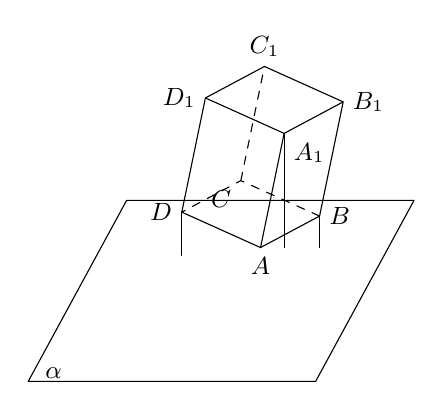
\begin{tikzpicture}[line cap=round,line join=round,font=\small]
  \coordinate (A)  at (1.25,0.35);
  \coordinate (B)  at (2.00,0.75);
  \coordinate (C)  at (1.00,1.20);
  \coordinate (D)  at (0.25,0.80);
  \coordinate (A1) at (1.55,1.80);
  \coordinate (B1) at (2.30,2.20);
  \coordinate (C1) at (1.30,2.65);
  \coordinate (D1) at (0.55,2.25);

  % 平面 α：A 位于其上，边界按源图作透视示意。
  \draw (-0.45,0.95)--(3.20,0.95)--(1.95,-1.35)--(-1.70,-1.35)--cycle;

  % 立方体可见棱与遮挡棱。
  \draw (D)--(A)--(B);
  \draw[dashed] (B)--(C)--(D);
  \draw (D)--(D1) (A)--(A1) (B)--(B1);
  \draw[dashed] (C)--(C1);
  \draw (D1)--(C1)--(B1)--(A1)--cycle;

  % 相邻顶点到平面 α 的距离线，仅作源图中的位置示意，不标尺寸。
  \draw[thin] (D)--(0.25,0.25);
  \draw[thin] (B)--(2.00,0.35);
  \draw[thin] (A1)--(1.55,0.35);

  \node[below] at (A) {$A$};
  \node[right] at (B) {$B$};
  \node[below left] at (C) {$C$};
  \node[left] at (D) {$D$};
  \node[below right] at (A1) {$A_1$};
  \node[right] at (B1) {$B_1$};
  \node[above] at (C1) {$C_1$};
  \node[left] at (D1) {$D_1$};
  \node[below left] at (-1.15,-1.05) {$\alpha$};
\end{tikzpicture}
\end{center}
\nopagebreak[4]
\Needspace{4\baselineskip}
\textbf{解析}

取从顶点 $A$ 出发的三条棱方向为坐标方向，并把到平面 $\alpha$ 的同侧有向距离记为线性函数。三个相邻顶点的距离为 $1,2,4$；其余四个顶点对应坐标位移分别为两两相加及三者相加，所以距离为 $3,5,6,7$。给出的候选数中 3、5、6、7 对应编号①、③、④、⑤，4 不可能，填①③④⑤。

\gkanswer{答案：①、③、④、⑤。}

\end{answer}
\begin{answer}
\gksolhead{17}{}

\textbf{题目}：

已知 $\dfrac{3\pi}{4}<\alpha<\pi$，$\tan\alpha+\cot\alpha=-\dfrac{10}{3}$。

（1） 求 $\tan\alpha$ 的值；

\Needspace{5\baselineskip}
（2） 求
\nopagebreak[4]
\[
\dfrac{5\sin^2\dfrac{\alpha}{2}+8\sin\dfrac{\alpha}{2}\cos\dfrac{\alpha}{2}+11\cos^2\dfrac{\alpha}{2}-8}{\sqrt{2}\sin\left(\alpha-\dfrac{\pi}{2}\right)}
\]
的值。

\Needspace{4\baselineskip}
\textbf{解析}

\gksubpart{(1)}

\Needspace{5\baselineskip}
令 $t=\tan\alpha$。方程 $t+1/t=-10/3$ 等价于
\nopagebreak[4]
\[
3t^2+10t+3=0,
\]
得 $t=-1/3$ 或 $t=-3$。由 $3\pi/4<\alpha<\pi$ 知 $-1<\tan\alpha<0$，故 $\tan\alpha=-1/3$。

\gksubpart{(2)}

\Needspace{5\baselineskip}
由 $\tan\alpha=-1/3$ 且 $\alpha$ 在第二象限，得
\nopagebreak[4]
\[
\sin\alpha=\frac1{\sqrt{10}},\qquad \cos\alpha=-\frac3{\sqrt{10}}.
\]
\Needspace{5\baselineskip}
令 $u=\sin(\alpha/2)$、$v=\cos(\alpha/2)$，则 $u^2=(1-\cos\alpha)/2$、$v^2=(1+\cos\alpha)/2$、$uv=\sin\alpha/2$。分子为
\nopagebreak[4]
\[
5u^2+8uv+11v^2-8=3\cos\alpha+4\sin\alpha=-\frac5{\sqrt{10}}.
\]
分母为 $\sqrt2\sin(\alpha-\pi/2)=-\sqrt2\cos\alpha=3\sqrt2/\sqrt{10}$，故所求为 $-5/(3\sqrt2)$。

\gkanswer{答案（1）：$-\dfrac13$。}

\gkanswer{答案（2）：$-\dfrac{5}{3\sqrt2}$。}

\end{answer}
\begin{answer}
\gksolhead{18}{}

\textbf{题目}：

在添加剂的搭配适用中，为了找到最佳的搭配方案，需要对各种不同的搭配方式作比较。在试制某种牙膏新品种时，需要选用两种不同的添加剂。现有芳香度分别为 $0,1,2,3,4,5$ 的六种添加剂可供选用。根据实验设计学原理，通常首先要随机选取两种不同的添加剂进行搭配实验。用 $\xi$ 表示所选用的两种不同的添加剂的芳香度之和。

（1） 写出 $\xi$ 的分布列；（以列表的形式给出结论，不必写计算过程）

（2） 求 $\xi$ 的数学期望 $E\xi$。（要求写出计算过程或说明道理）

\Needspace{4\baselineskip}
\textbf{解析}

任取六种芳香度 $0,1,2,3,4,5$ 中的两种不同添加剂，共有 $\binom62=15$ 个等可能无序组合。各组合芳香度之和从 1 到 9 的出现次数依次为 $1,1,2,2,3,2,2,1,1$。

\gksubpart{(1)}

\Needspace{5\baselineskip}
因此 $\xi=1,2,\ldots,9$ 的概率依次为
\nopagebreak[4]
\[
\frac1{15},\frac1{15},\frac2{15},\frac2{15},\frac3{15},
\frac2{15},\frac2{15},\frac1{15},\frac1{15}.
\]

\gksubpart{(2)}

\Needspace{5\baselineskip}
六个数的总和为 $15$。两两无序取样中，每个数出现在五个组合里，所以所有组合和的总和为 $5\cdot15=75$。故
\nopagebreak[4]
\[
E\xi=\frac{75}{15}=5.
\]

\gkanswer{答案（1）：当 $\xi=1,2,\ldots,9$ 时，其概率依次为 $\dfrac1{15},\dfrac1{15},\dfrac2{15},\dfrac2{15},\dfrac3{15},\dfrac2{15},\dfrac2{15},\dfrac1{15},\dfrac1{15}$。}

\gkanswer{答案（2）：$E\xi=5$。}

\end{answer}
\begin{answer}
\gksolhead{19}{}

\textbf{题目}：

如图，$P$ 是边长为 $1$ 的正六边形 $ABCDEF$ 所在平面外一点，$PA=1$，$P$ 在平面 $ABC$ 内的射影为 $BF$ 的中点 $O$。

（1） 证明：$PA\perp BF$；

（2） 求面 $APB$ 与面 $DPB$ 所成二面角的大小。
\nopagebreak[4]
\begin{center}% 2006 安徽卷理 Q19；正六边形及空间点的仿射投影示意，O 为 BF 中点。
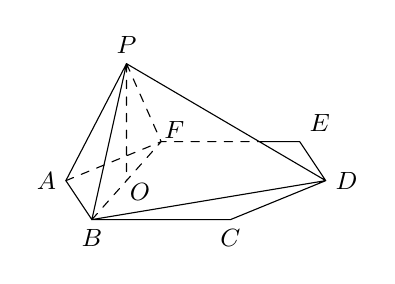
\begin{tikzpicture}[scale=1.1,line cap=round,line join=round,font=\small]
  \coordinate (A) at (0,0);
  \coordinate (B) at (0.3,-0.45);
  \coordinate (C) at (1.9,-0.45);
  \coordinate (D) at (3,0);
  \coordinate (E) at (2.7,0.45);
  \coordinate (F) at (1.1,0.45);
  \coordinate (H) at (2.2333333,0.45); % PD 与 FE 的图示交点，仅用于分段绘线
  \coordinate (O) at (0.7,0);
  \coordinate (P) at (0.7,1.35);

  \draw[dashed] (A)--(F)--(H) (B)--(F) (P)--(F) (P)--(O);
  \draw (H)--(E) (A)--(B)--(C)--(D)--(E) (B)--(D) (P)--(A) (P)--(B) (P)--(D);

  \node[left] at (A) {$A$};
  \node[below] at (B) {$B$};
  \node[below] at (C) {$C$};
  \node[right] at (D) {$D$};
  \node[above right] at (E) {$E$};
  \node[above right,inner sep=1pt] at (F) {$F$};
  \node[below right,inner sep=1pt] at (O) {$O$};
  \node[above] at (P) {$P$};
\end{tikzpicture}
\end{center}
\nopagebreak[4]
\Needspace{4\baselineskip}
\textbf{解析}

\Needspace{5\baselineskip}
在正六边形所在平面取坐标
\nopagebreak[4]
\[
A=(1,0,0),\quad B=(\tfrac12,\tfrac{\sqrt3}{2},0),\quad
D=(-1,0,0),\quad F=(\tfrac12,-\tfrac{\sqrt3}{2},0).
\]
则 $O$ 为 $BF$ 中点，$O=(\tfrac12,0,0)$。由于 $PO$ 垂直于底面，且 $PA=1$、$AO=1/2$，可取 $P=(\tfrac12,0,\tfrac{\sqrt3}{2})$；镜像情形结果相同。

\gksubpart{(1)}

$\overrightarrow{AP}=(-\tfrac12,0,\tfrac{\sqrt3}{2})$，$\overrightarrow{BF}=(0,-\sqrt3,0)$，两者点积为 $0$，所以 $PA\perp BF$。

\gksubpart{(2)}

\Needspace{5\baselineskip}
沿公共棱 $PB$ 作垂直截面。取分别朝向 $A$、$D$ 的两个半平面，其截线方向是 $\overrightarrow{BA}$、$\overrightarrow{BD}$ 在垂直于 $PB$ 平面上的正交投影。令
\nopagebreak[4]
\[
\mathbf u=(\tfrac12,-\tfrac{\sqrt3}{4},-\tfrac{\sqrt3}{4}),\qquad
\mathbf v=(-\tfrac32,-\tfrac{\sqrt3}{4},-\tfrac{\sqrt3}{4}).
\]
\Needspace{5\baselineskip}
则 $\mathbf u\cdot\mathbf v=-3/8$，$|\mathbf u|^2=5/8$，$|\mathbf v|^2=21/8$，所以
\nopagebreak[4]
\[
\cos\theta=\frac{\mathbf u\cdot\mathbf v}{|\mathbf u||\mathbf v|}
=-\frac3{\sqrt{105}}.
\]
按包含 $A,D$ 的两个半平面，二面角为 $\arccos(-3/\sqrt{105})$。

两平面的较小夹角为其补角 $\arccos(3/\sqrt{105})$；固定 PDF 无答案页，角度约定无法确认。

\gkanswer{答案（1）：见解析版。}

\gkanswer{答案（2）：按包含 $A,D$ 的两个半平面，二面角为 $\arccos\left(-\dfrac3{\sqrt{105}}\right)$；若取两平面间的较小夹角，则为其补角。}

\end{answer}
\begin{answer}
\gksolhead{20}{}

\textbf{题目}：

\Needspace{5\baselineskip}
已知函数 $f(x)$ 在 $\mathbb R$ 上有定义，对任意实数 $a>0$ 和任意实数 $x$，都有
\nopagebreak[4]
\[
f(ax)=af(x)\text{。}
\]

（1） 证明 $f(0)=0$；

\Needspace{5\baselineskip}
（2） 证明
\nopagebreak[4]
\[
f(x)=\begin{cases}
kx,&x\geqslant0,\\
hx,&x<0,
\end{cases}
\]
其中 $k$ 和 $h$ 均为常数；

（3） 当（2）中的 $k>0$ 时，设 $g(x)=\dfrac{1}{f(x)}+f(x)$（$x>0$），讨论 $g(x)$ 在 $(0,+\infty)$ 内的单调性并求极值。

\Needspace{4\baselineskip}
\textbf{解析}

\gksubpart{(1)}

在 $f(ax)=af(x)$ 中取 $x=0$，并选任意 $a>0$ 且 $a\ne1$，得 $f(0)=af(0)$，故 $f(0)=0$。

\gksubpart{(2)}

令 $k=f(1)$。若 $x>0$，取原条件中的 $a=x$、自变量为 $1$，得 $f(x)=xf(1)=kx$；当 $x=0$ 时该式也成立。再令 $h=-f(-1)$。若 $x<0$，取 $a=-x>0$、自变量为 $-1$，得 $f(x)=(-x)f(-1)=hx$。所以题设分段式成立。

\gksubpart{(3)}

\Needspace{5\baselineskip}
当 $x>0$ 时 $f(x)=kx$，所以
\nopagebreak[4]
\[
g(x)=kx+\frac1{kx},\qquad
g'(x)=k-\frac1{kx^2}.
\]
当 $0<x<1/k$ 时导数为负；当 $x>1/k$ 时导数为正。因此 $g$ 在 $(0,1/k]$ 上递减，在 $[1/k,+\infty)$ 上递增，最小值为 $g(1/k)=2$，无最大值。

\gkanswer{答案（1）：$f(0)=0$。}

\gkanswer{答案（2）：$f(x)=\begin{cases}kx,&x\geqslant0,\\hx,&x<0,\end{cases}$，其中 $k,h$ 为常数。}

\gkanswer{答案（3）：在 $(0,1/k]$ 上递减，在 $[1/k,+\infty)$ 上递增；最小值为 $2$，在 $x=1/k$ 处取得，无最大值。}

\end{answer}
\begin{answer}
\gksolhead{21}{}

\textbf{题目}：

数列 $\{a_n\}$ 的前 $n$ 项和为 $S_n$，已知 $a_1=\dfrac12$，$S_n=n^2a_n-n(n-1)$，$n=1,2,\ldots$。

（1） 写出 $S_n$ 与 $S_{n-1}$ 的递推关系式（$n\geqslant2$），并求 $S_n$ 关于 $n$ 的表达式；

（2） 设 $f_n(x)=\dfrac{S_n}{n}x^{n+1}$，$b_n=f_n'(p)$（$p\in\mathbb R$），求数列 $\{b_n\}$ 的前 $n$ 项和 $T_n$。

\Needspace{4\baselineskip}
\textbf{解析}

\gksubpart{(1)}

\Needspace{5\baselineskip}
由 $a_n=S_n-S_{n-1}$ 及题设
\nopagebreak[4]
\[
S_n=n^2(S_n-S_{n-1})-n(n-1),
\]
\Needspace{5\baselineskip}
整理得
\nopagebreak[4]
\[
(n^2-1)S_n=n^2S_{n-1}+n(n-1),
\]
\Needspace{5\baselineskip}
即
\nopagebreak[4]
\[
S_n=\frac{n^2}{n^2-1}S_{n-1}+\frac{n}{n+1}\quad(n\ge2).
\]
\Needspace{5\baselineskip}
令 $T_n=(n+1)S_n/n$，则由递推式
\nopagebreak[4]
\[
T_n=\frac{n}{n-1}S_{n-1}+1=T_{n-1}+1.
\]
又 $S_1=a_1=1/2$，故 $T_1=1$，从而 $T_n=n$，即 $S_n=n^2/(n+1)$。

\gksubpart{(2)}

\nopagebreak[4]
\[
f_n(x)=\frac{S_n}{n}x^{n+1}=\frac{n}{n+1}x^{n+1},
\qquad b_n=f_n'(p)=np^n.
\]
\Needspace{5\baselineskip}
当 $p\ne1$，利用有限几何级数求导可得
\nopagebreak[4]
\[
T_n=\sum_{k=1}^n kp^k
=\frac{p\left[1-(n+1)p^n+np^{n+1}\right]}{(1-p)^2}.
\]
当 $p=1$ 时，$T_n=\sum_{k=1}^n k=n(n+1)/2$。

\gkanswer{答案（1）：$S_n=\dfrac{n^2}{n+1}$，递推关系为 $S_n=\dfrac{n^2}{n^2-1}S_{n-1}+\dfrac{n}{n+1}$（$n\geqslant2$）。}

\gkanswer{答案（2）：$T_n=\dfrac{p\left[1-(n+1)p^n+np^{n+1}\right]}{(1-p)^2}$（$p\ne1$）；$p=1$ 时 $T_n=\dfrac{n(n+1)}2$。}

\end{answer}
\begin{answer}
\gksolhead{22}{}

\textbf{题目}：

如图，$F$ 为双曲线 $C\text{：}\dfrac{x^2}{a^2}-\dfrac{y^2}{b^2}=1$（$a>0,b>0$）的右焦点，$P$ 为双曲线 $C$ 右支上一点，且位于 $x$ 轴上方，$M$ 为左准线上一点，$O$ 为坐标原点。已知四边形 $OFPM$ 为平行四边形，$|PF|=\lambda|OF|$。

（1） 写出双曲线 $C$ 的离心率 $e$ 与 $\lambda$ 的关系式；

（2） 当 $\lambda=1$ 时，经过焦点 $F$ 且平行于 $OP$ 的直线交双曲线于 $A,B$ 点，若 $|AB|=12$，求此时的双曲线方程。
\nopagebreak[4]
\begin{center}% 2006 安徽卷理 Q22；取 a=1、e=2 作满足题设几何关系的示意。
\begin{tikzpicture}[x=0.9cm,y=0.72cm,line cap=round,line join=round,>=stealth,font=\small]
  \coordinate (O) at (0,0);
  \coordinate (F) at (2,0);
  \coordinate (M) at (-0.5,{sqrt(15)/2});
  \coordinate (P) at (1.5,{sqrt(15)/2});
  \draw[->] (-3.4,0)--(3.5,0) node[right] {$x$};
  \draw[->] (0,-3.7)--(0,3.9) node[above] {$y$};
  \draw (-0.5,-3.1)--(-0.5,3.1);
  \draw[thick,domain=-3.4:3.4,samples=100] plot ({sqrt(1+\x*\x/3)},\x);
  \draw[thick,domain=-3.4:3.4,samples=100] plot ({-sqrt(1+\x*\x/3)},\x);
  \draw (O)--(M)--(P)--(F);
  \node[below right] at (O) {$O$};
  \node[below] at (F) {$F$};
  \node[left] at (M) {$M$};
  \node[above left] at (P) {$P$};
\end{tikzpicture}
\end{center}
\nopagebreak[4]
\Needspace{4\baselineskip}
\textbf{解析}

\gksubpart{(1)}

记焦半径参数为 $c$，则 $c=ae$、$b^2=c^2-a^2$。左准线为 $x=-a/e$。按四边形 $OFPM$ 的顶点顺序，$OFPM$ 为平行四边形意味着 $P=F+M$；故 $x_P=c-a/e$。因 $P$ 在右支上，须 $x_P>a$，所以 $e-1/e>1$，即 $e>(1+\sqrt5)/2$。

\Needspace{5\baselineskip}
由双曲线焦点—准线定义，右焦点 $F$ 到 $P$ 的距离为 $e$ 倍的 $P$ 到右准线的距离：
\nopagebreak[4]
\[
|PF|=e\left(x_P-\frac ae\right)=e(c-a/e)-a=ec-2a.
\]
\Needspace{5\baselineskip}
又 $|PF|=\lambda|OF|=\lambda c$，于是
\nopagebreak[4]
\[
\lambda=e-\frac2e,\qquad
e=\frac{\lambda+\sqrt{\lambda^2+8}}2.
\]

\gksubpart{(2)}

\Needspace{5\baselineskip}
当 $\lambda=1$ 时 $e-2/e=1$，取 $e>1$ 的解得 $e=2$，故 $c=2a$、$b^2=3a^2$。由平行四边形关系，
\nopagebreak[4]
\[
P=(c-a/e,y_P)=(\tfrac32a,y_P).
\]
代入双曲线方程并用 $b^2=3a^2$，得 $y_P=\sqrt{15}a/2$，所以直线 $OP$ 的方向向量可取 $(3,\sqrt{15})$。

\Needspace{5\baselineskip}
过 $F=(2a,0)$ 且平行于 $OP$ 的直线可参数化为
\nopagebreak[4]
\[
(x,y)=(2a,0)+t(3,\sqrt{15}).
\]
\Needspace{5\baselineskip}
代入 $x^2/a^2-y^2/(3a^2)=1$ 得
\nopagebreak[4]
\[
4t^2+12at+3a^2=0.
\]
两交点的参数差为 $\sqrt6a$，方向向量长为 $\sqrt{24}$，故弦长为 $12a$。由 $|AB|=12$ 得 $a=1$、$b^2=3$，所求双曲线方程为 $x^2-y^2/3=1$。

\gkanswer{答案（1）：$\lambda=e-\dfrac2e$，即 $e=\dfrac{\lambda+\sqrt{\lambda^2+8}}2$；由 $P$ 位于右支且在 $x$ 轴上方，还须 $e>\dfrac{1+\sqrt5}{2}$。}

\gkanswer{答案（2）：$x^2-\dfrac{y^2}{3}=1$。}

\end{answer}